\newcommand{\malwareResultsAucTable}{
    \begin{table}[H]
        \centering
        \begin{tabular}{|p{2,8cm}||p{2,8cm} p{2,8cm} p{2,8cm}|}
            \hline
            Malware Label & ALOHA & Joint Embedding & Proposed Model \\
            \hline
            AUC-ROC & \textBF{0.994$\pm$0.000} & - & \textBF{0.994$\pm$0.000} \\
            \hline
        \end{tabular}
        \caption{AUC-ROC (Area Under Curve) of the different models for the \textbf{Malware Label} prediction task. Results were aggregated over \textBF{3} training runs with different weight initializations and minibatch orderings. Best results are shown in \textbf{bold}.} \label{tab:malware_auc}
    \end{table}
}

\newcommand{\malwareResultsAtFprTable}{
    \begin{center}
        \begin{longtable}[c]{|p{3,2cm}||p{1,8cm} p{1,8cm} p{1,8cm} p{1,8cm} p{1,8cm}|}
            \hline
            Malware Label & \multicolumn{5}{c|}{{FPR}} \\
            & $10^{-5}$ & $10^{-4}$ & $10^{-3}$ & $10^{-2}$ & $10^{-1}$ \\
            \hline
            \endfirsthead

            \caption*{\raggedright ...continued from previous page} \\
            \hline
            Malware Label & \multicolumn{5}{c|}{\textbf{FPR}} \\
            & $10^{-5}$ & $10^{-4}$ & $10^{-3}$ & $10^{-2}$ & $10^{-1}$ \\
            \hline
            \endhead

            \caption*{\raggedleft ...continued on next page} \\
            \endfoot

            \caption{Mean and standard deviation results (TPR, Accuracy, Recall, Precision and F1-Score) of the different models for the \textbf{Malware Label} prediction task at different \textbf{FPR}s (\textit{False Positive Rates}). Results were aggregated over \textBF{3} training runs with different weight initializations and minibatch orderings. Best results are shown in \textbf{bold}. Under \textbf{TPR} results are also presented the percentage reduction in mean detection error and in ROC curve standard deviation introduced by the \textit{Proposed Model} with respect to both \textit{ALOHA} model and \textit{Joint Embedding}.} \label{tab:malware_results_at_fpr} \\
            \endlastfoot

            \multicolumn{6}{|c|}{\textbf{TPR}} \\
            \hline
            ALOHA & \textBF{0.604$\pm$0.022} & \textBF{0.752$\pm$0.010} & 0.880$\pm$0.009 & \textBF{0.957$\pm$0.006} & 0.985$\pm$0.003 \\
            Joint Embedding & - & - & - & - & - \\
            Proposed Model & 0.579$\pm$0.027 & 0.752$\pm$0.015 & \textBF{0.890$\pm$0.005} & 0.951$\pm$0.003 & \textBF{0.988$\pm$0.003} \\
            \hline
            Error Reduction wrt \newline ALOHA & -6.3\% & 0.0\% & 8.3\% & -14.0\% & 20.0\% \\
            Error Reduction wrt \newline Joint Embedding & - & - & - & - & - \\
            \hline
            Std Reduction wrt \newline ALOHA & -22.7\% & -50.0\% & 44.4\% & 50.0\% & 0.0\% \\
            Std Reduction wrt \newline Joint Embedding & - & - & - & - & - \\
            \hline
            \multicolumn{6}{|c|}{\textbf{Accuracy}} \\
            \hline
            ALOHA & \textBF{0.847$\pm$0.008} & \textBF{0.904$\pm$0.004} & 0.953$\pm$0.004 & \textBF{0.977$\pm$0.002} & 0.933$\pm$0.001 \\
            Joint Embedding & - & - & - & - & - \\
            Proposed Model & 0.837$\pm$0.010 & 0.904$\pm$0.006 & \textBF{0.957$\pm$0.002} & 0.975$\pm$0.001 & \textBF{0.934$\pm$0.001} \\
            \hline
            \multicolumn{6}{|c|}{\textbf{Recall}} \\
            \hline
            ALOHA & \textBF{0.604$\pm$0.022} & \textBF{0.752$\pm$0.010} & 0.880$\pm$0.009 & \textBF{0.957$\pm$0.006} & 0.985$\pm$0.003 \\
            Joint Embedding & - & - & - & - & - \\
            Proposed Model & 0.579$\pm$0.027 & 0.752$\pm$0.015 & \textBF{0.890$\pm$0.005} & 0.951$\pm$0.003 & \textBF{0.988$\pm$0.003} \\
            \hline
            \multicolumn{6}{|c|}{\textbf{Precision}} \\
            \hline
            ALOHA & \textBF{1.000$\pm$0.000} & \textBF{1.000$\pm$0.000} & \textBF{0.998$\pm$0.000} & \textBF{0.984$\pm$0.000} & \textBF{0.862$\pm$0.000} \\
            Joint Embedding & - & - & - & - & - \\
            Proposed Model & \textBF{1.000$\pm$0.000} & \textBF{1.000$\pm$0.000} & \textBF{0.998$\pm$0.000} & \textBF{0.984$\pm$0.000} & \textBF{0.862$\pm$0.000} \\
            \hline
            \multicolumn{6}{|c|}{\textbf{F1 Score}} \\
            \hline
            ALOHA & \textBF{0.753$\pm$0.017} & \textBF{0.859$\pm$0.007} & 0.935$\pm$0.005 & \textBF{0.970$\pm$0.003} & 0.919$\pm$0.001 \\
            Joint Embedding & - & - & - & - & - \\
            Proposed Model & 0.733$\pm$0.022 & 0.858$\pm$0.009 & \textBF{0.941$\pm$0.003} & 0.967$\pm$0.002 & \textBF{0.921$\pm$0.001} \\
            \hline
        \end{longtable}
    \end{center}
}

\newcommand{\malwareResultsSummaryTable}{
    \begin{table}[H]
        \centering
        \begin{tabular}{|p{3,2cm}||p{1,8cm} p{1,8cm} p{1,8cm} p{1,8cm} p{1,8cm}|}
            \hline
            \multicolumn{6}{|c|}{Malware Label (at FPR $=1\%$)} \\
            \hline
            Model & TPR & Accuracy & Precision & Recall & F1 score \\
            \hline
            ALOHA & \textBF{0.957$\pm$0.006} & \textBF{0.977$\pm$0.002} & \textBF{0.984$\pm$0.000} & \textBF{0.957$\pm$0.006} & \textBF{0.970$\pm$0.003} \\
            Joint Embedding & - & - & - & - & - \\
            Proposed Model & 0.951$\pm$0.003 & 0.975$\pm$0.001 & \textBF{0.984$\pm$0.000} & 0.951$\pm$0.003 & 0.967$\pm$0.002 \\
            \hline
        \end{tabular}
        \caption{Summary of the mean and standard deviation results of the different models for the \textbf{Malware Label} prediction task at \textbf{FPR} $=1\%$. Results were aggregated over \textBF{3} training runs with different weight initializations and minibatch orderings. Best results are shown in \textbf{bold}.} \label{tab:malware_result_summary}
    \end{table}
}

\newcommand{\malwareRocAloha}{
    \begin{figure}[H]
        \vspace*{-0.5cm}
        \centering
        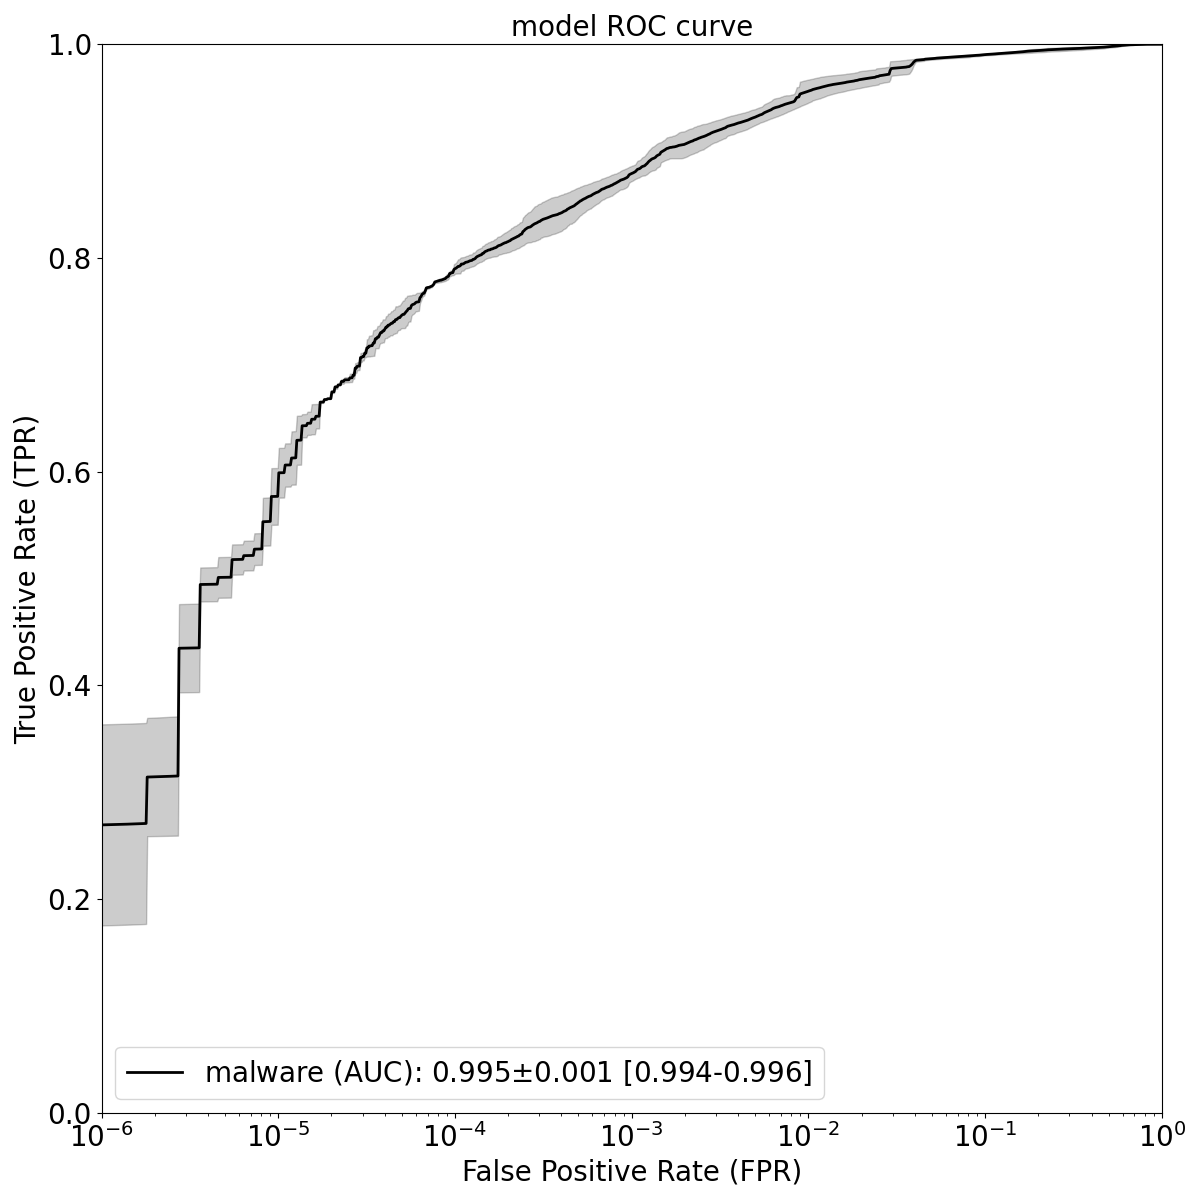
\includegraphics[width=0.6\textwidth]{./results/malware_roc_aloha.png}
        \vspace*{-0.2cm}
        \caption{ROC curve and AUC statistics of \textBF{ALOHA} model for the \textbf{Malware Label}. The line represents the \textit{mean} TPR at a given FPR, while the shaded region represents the \textit{standard deviation}. Statistics were computed over \textBF{3} training runs, each with random parameter initialization.}
        \label{fig:malwareRocAloha}
    \end{figure}
}

\newcommand{\malwareRocJointEmbedding}{
    \begin{figure}[H]
        \vspace*{-0.5cm}
        \centering
        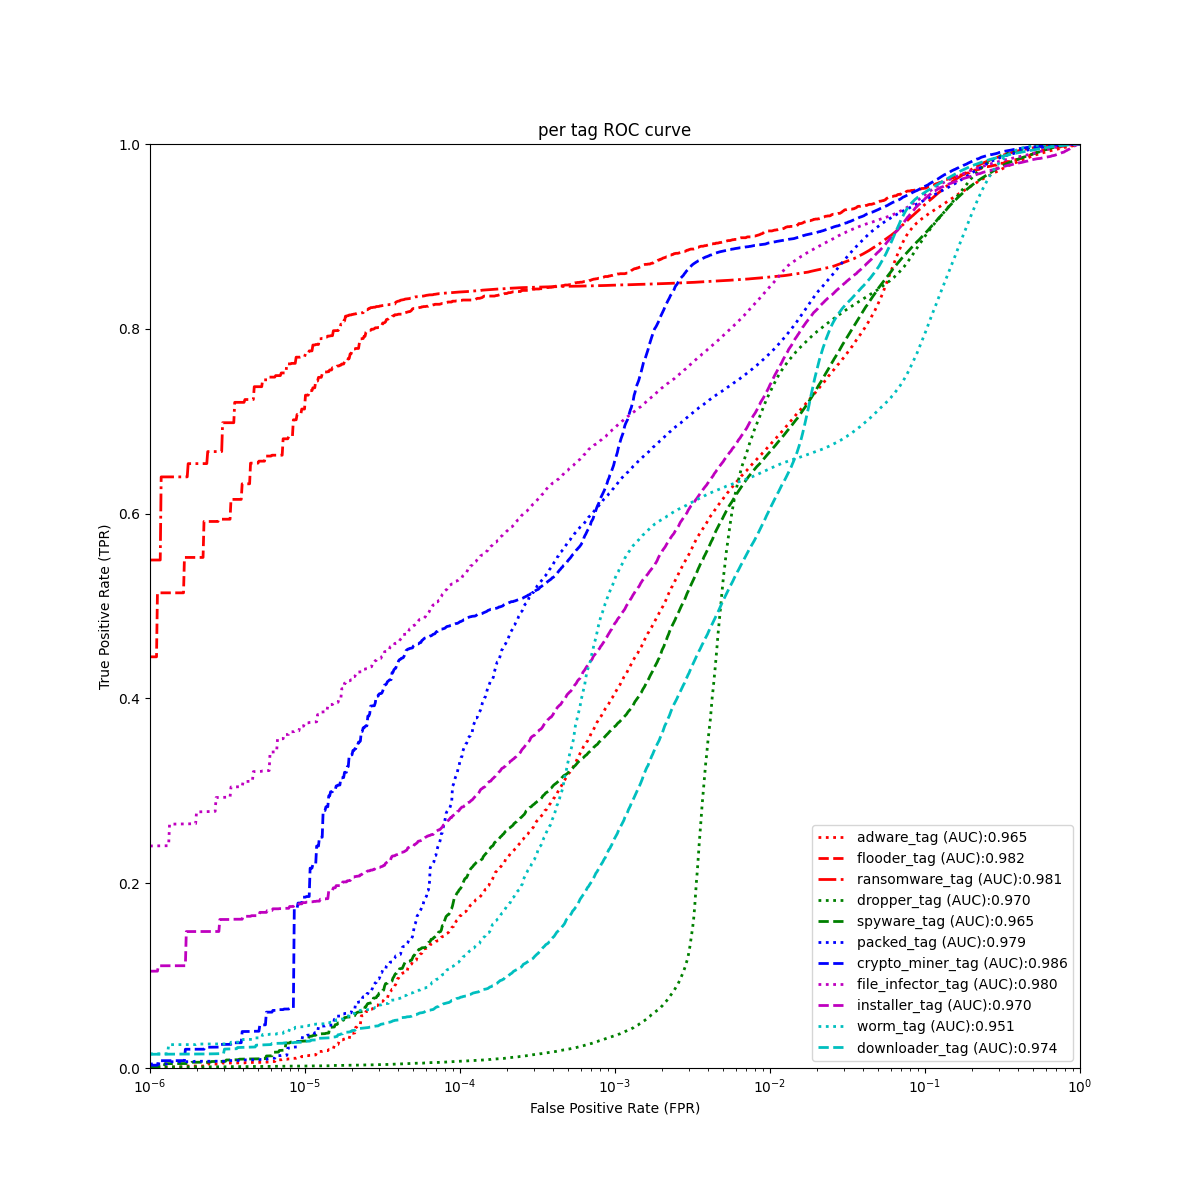
\includegraphics[width=0.6\textwidth]{./results/malware_roc_jointEmbedding.png}
        \vspace*{-0.2cm}
        \caption{ROC curve and AUC statistics of \textBF{Joint Embedding} model for the \textbf{Malware Label}. The line represents the \textit{mean} TPR at a given FPR, while the shaded region represents the \textit{standard deviation}. Statistics were computed over \textBF{3} training runs, each with random parameter initialization.}
        \label{fig:malwareRocJointEmbedding}
    \end{figure}
}

\newcommand{\malwareRocProposedMethod}{
    \begin{figure}[H]
        \vspace*{-0.5cm}
        \centering
        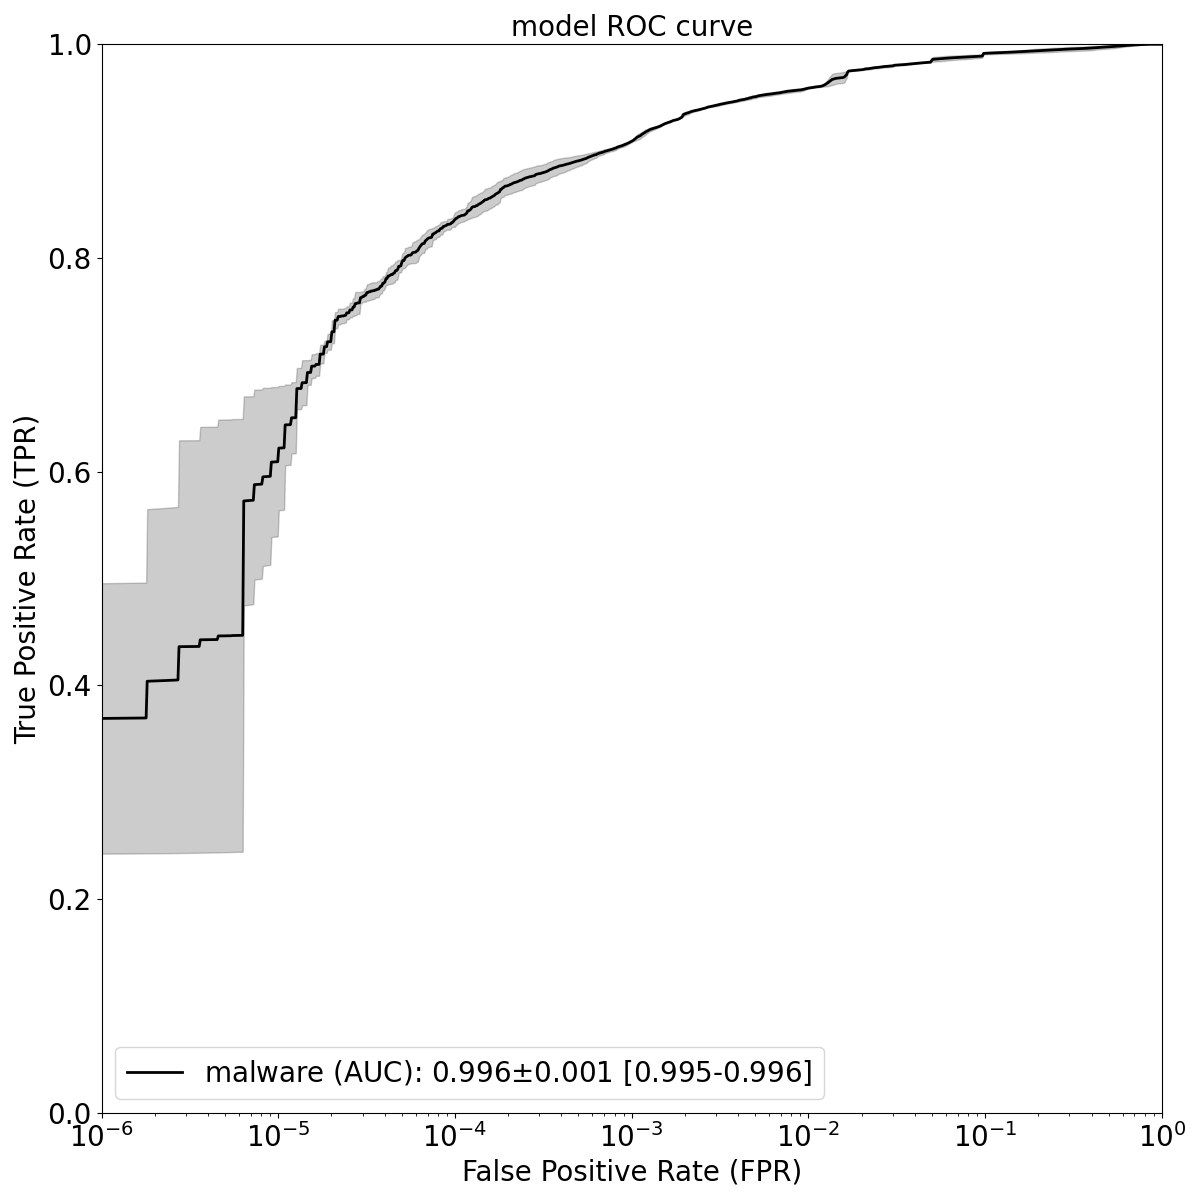
\includegraphics[width=0.6\textwidth]{./results/malware_roc_proposedModel.png}
        \vspace*{-0.2cm}
        \caption{ROC curve and AUC statistics of \textBF{Proposed Model} for the \textbf{Malware Label}. The line represents the \textit{mean} TPR at a given FPR, while the shaded region represents the \textit{standard deviation}. Statistics were computed over \textBF{3} training runs, each with random parameter initialization.}
        \label{fig:malwareRocProposedModel}
    \end{figure}
}
